\documentclass[aspectratio=169,11pt]{beamer}

\usepackage[utf8]{inputenc}
\usepackage[T1]{fontenc}
\usepackage[spanish,es-nodecimaldot]{babel}
\usepackage{amsmath,amssymb,mathtools}
\usepackage{booktabs}
\usepackage{colortbl}
\usepackage{graphicx}
\usepackage{xcolor}
\usepackage{hyperref}

\definecolor{navy}{HTML}{17324D}
\definecolor{teal}{HTML}{1F7A7A}
\definecolor{gold}{HTML}{D39B2A}
\definecolor{ink}{HTML}{263238}
\definecolor{mist}{HTML}{EEF3F5}
\definecolor{softred}{HTML}{B94A48}

\setbeamercolor{normal text}{fg=ink,bg=white}
\setbeamercolor{structure}{fg=teal}
\setbeamercolor{frametitle}{fg=white,bg=navy}
\setbeamercolor{title}{fg=white}
\setbeamercolor{subtitle}{fg=white!82}
\setbeamercolor{block title}{fg=white,bg=teal}
\setbeamercolor{block body}{fg=ink,bg=mist}
\setbeamercolor{alerted text}{fg=softred}
\setbeamertemplate{navigation symbols}{}
\setbeamertemplate{itemize item}{\color{teal}$\blacksquare$}
\setbeamertemplate{itemize subitem}{\color{gold}$\blacktriangleright$}
\setbeamertemplate{footline}{%
  \leavevmode\hbox{%
  \begin{beamercolorbox}[wd=.82\paperwidth,ht=2.7ex,dp=1.2ex,leftskip=1em]{author in head/foot}%
    \color{navy}\scriptsize Acemoglu y Restrepo: la carrera entre el hombre y la máquina
  \end{beamercolorbox}%
  \begin{beamercolorbox}[wd=.18\paperwidth,ht=2.7ex,dp=1.2ex,rightskip=1em plus1fil]{date in head/foot}%
    \color{navy}\scriptsize\hfill\insertframenumber/\inserttotalframenumber
  \end{beamercolorbox}}}
\setbeamertemplate{headline}{}

\newcommand{\key}[1]{\textcolor{teal}{\textbf{#1}}}
\newcommand{\source}[1]{\vfill\hfill{\tiny\color{gray}#1}}

\title{La carrera entre el hombre y la máquina}
\subtitle{Automatización, productividad, salarios y participación laboral}
\author{Alexander Quispe}
\institute{IA y Modelamiento Económico}
\date{Tarea 5 --- 2026}

\begin{document}

\begin{frame}[plain]
  \begin{beamercolorbox}[wd=\paperwidth,ht=\paperheight,dp=0ex,sep=1.15cm]{frametitle}
    \vspace{0.45cm}
    {\usebeamerfont{title}\LARGE\bfseries\inserttitle\par}
    \vspace{0.25cm}
    {\large\insertsubtitle\par}
    \vspace{1.05cm}
    {\normalsize\insertauthor\par}
    {\small\insertinstitute\par}
    \vspace{0.65cm}
    {\small\href{https://github.com/isisroquet-mi/ai-06-restrepo}{github.com/isisroquet-mi/ai-06-restrepo}\par}
    \vfill
    {\small\insertdate\par}
  \end{beamercolorbox}
\end{frame}

\begin{frame}{La pregunta económica}
  \begin{columns}[T,onlytextwidth]
    \column{0.48\textwidth}
      \begin{block}{La tecnología actúa sobre tareas}
        La automatización permite que el capital realice tareas antes asignadas al trabajo.
        La creación de nuevas tareas abre actividades en las que el trabajo conserva ventaja.
      \end{block}
    \column{0.48\textwidth}
      \begin{block}{El efecto agregado combina dos fuerzas}
        \key{Productividad}: producir lo mismo cuesta menos.

        \key{Desplazamiento}: el trabajo pierde parte de su rango de tareas.
      \end{block}
  \end{columns}
  \vspace{0.45cm}
  \centering
  \Large La productividad puede aumentar mientras el salario disminuye.
  \source{Acemoglu y Restrepo (2018), introducción y Proposición 3.}
\end{frame}

\begin{frame}{Un continuo de tareas organiza la producción}
  \centering
  \begin{tabular}{p{0.12\textwidth}p{0.30\textwidth}p{0.08\textwidth}p{0.30\textwidth}p{0.12\textwidth}}
    \multicolumn{1}{c}{$N-1$} &
    \multicolumn{1}{c}{\cellcolor{navy!12}\textbf{Capital}} &
    \multicolumn{1}{c}{$I^{*}$} &
    \multicolumn{1}{c}{\cellcolor{teal!13}\textbf{Trabajo}} &
    \multicolumn{1}{c}{$N$} \\
  \end{tabular}
  \vspace{0.7cm}
  \begin{columns}[T,onlytextwidth]
    \column{0.48\textwidth}
      \key{Automatización:} un aumento de $I$ desplaza $I^{*}$ cuando la tecnología restringe la asignación.
      El capital absorbe más tareas existentes.
    \column{0.48\textwidth}
      \key{Nuevas tareas:} un aumento de $N$ amplía el extremo intensivo en trabajo.
      El trabajo recupera tareas en las que tiene ventaja comparativa.
  \end{columns}
  \vspace{0.55cm}
  \[
    I^{*}=\min\{I,\widetilde I\}.
  \]
  \source{Modelo estático, secciones 2.1--2.3.}
\end{frame}

\begin{frame}{El equilibrio conecta decisiones y precios}
  \begin{columns}[T,onlytextwidth]
    \column{0.31\textwidth}
      \begin{block}{Hogares}
        Ofrecen trabajo, ahorran y poseen el capital. La elasticidad $\varepsilon_L$ resume la respuesta de la oferta laboral.
      \end{block}
    \column{0.31\textwidth}
      \begin{block}{Empresas}
        Asignan cada tarea al factor de menor costo efectivo y demandan capital y trabajo.
      \end{block}
    \column{0.31\textwidth}
      \begin{block}{Tecnología}
        $\gamma(i)$ mide la ventaja comparativa del trabajo. $I$ limita la automatización y $N$ determina la frontera de tareas.
      \end{block}
  \end{columns}
  \vspace{0.45cm}
  \begin{itemize}
    \item Los precios de equilibrio son el salario $W$ y la renta del capital $R$.
    \item La razón $\omega=W/R$ determina la tarea marginal que cambia de factor.
    \item La elasticidad relevante depende de si la tecnología restringe esa reasignación.
  \end{itemize}
  \source{Ecuaciones (1)--(13) y Proposición 2.}
\end{frame}

\begin{frame}{Automatización y nuevas tareas tienen efectos opuestos}
  \begin{columns}[T,onlytextwidth]
    \column{0.48\textwidth}
      \begin{block}{Más automatización: $dI>0$}
        \begin{itemize}
          \item Reduce $W/R$ cuando $I^{*}=I<\widetilde I$.
          \item Reduce la participación laboral y el empleo.
          \item Aumenta la productividad, pero el salario queda ambiguo.
        \end{itemize}
      \end{block}
    \column{0.48\textwidth}
      \begin{block}{Más nuevas tareas: $dN>0$}
        \begin{itemize}
          \item Aumenta $W/R$.
          \item Aumenta la participación laboral y el empleo.
          \item Aumenta la productividad y el salario.
        \end{itemize}
      \end{block}
  \end{columns}
  \vspace{0.35cm}
  \centering
  \large El resultado depende de qué lado de la ``carrera'' avanza más rápido.
  \source{Proposiciones 2 y 3.}
\end{frame}

\begin{frame}{Proposición 3: supuestos, casos y conclusión}
  \small
  \key{Supuestos:} se cumplen los Supuestos 1, 2 y 3; $d\ln Y\vert_{K,L}$ mide el cambio de productividad manteniendo $K$ y $L$ constantes.
  \vspace{0.3cm}
  \begin{columns}[T,onlytextwidth]
    \column{0.49\textwidth}
      \begin{block}{$I^{*}=I<\widetilde I$}
        $W/\gamma(I^{*})>R>W/\gamma(N)$.

        Automatización y nuevas tareas elevan la productividad.

        $N$ eleva el salario. $I$ eleva la renta del capital, pero su efecto salarial es ambiguo. Existe un umbral de capital que cambia el signo.
      \end{block}
    \column{0.49\textwidth}
      \begin{block}{$I^{*}=\widetilde I<I$}
        $W/\gamma(I^{*})=R>W/\gamma(N)$.

        La automatización adicional no cambia productividad ni precios porque la asignación ya no está restringida por $I$.

        Las nuevas tareas elevan productividad y salario.
      \end{block}
  \end{columns}
  \source{NBER Working Paper 22252, Proposición 3, pp. 12--14.}
\end{frame}

\begin{frame}{Salario y participación laboral son objetos distintos}
  \begin{columns}[T,onlytextwidth]
    \column{0.48\textwidth}
      \begin{block}{Participación laboral}
        En el caso restringido, la automatización reduce $W/R$.
        Por eso la participación del trabajo cae de forma no ambigua.
      \end{block}
    \column{0.48\textwidth}
      \begin{block}{Salario real}
        El salario combina el aumento de productividad con la pérdida de tareas.
        Su signo depende de cuál fuerza domina.
      \end{block}
  \end{columns}
  \vspace{0.55cm}
  \[
    \underbrace{d\ln W}_{\text{salario}}
    =\underbrace{d\ln Y\vert_{K,L}}_{\text{productividad}}
    -\underbrace{(1-s_L)\frac{\Lambda_I}{\widehat\sigma+\varepsilon_L}\,dI}_{\text{desplazamiento}}.
  \]
  \centering
  \large Una menor participación laboral no implica necesariamente un menor salario.
  \source{Proposición 3 y discusión posterior.}
\end{frame}

\begin{frame}{Derivación manual: el efecto productividad}
  Para automatización marginal con $I^{*}=I<\widetilde I$ y $dN=0$, defino
  \[
    P_I=\frac{B^{\widehat\sigma-1}}{1-\widehat\sigma}
    \left[
      \left(\frac{W}{\gamma(I)}\right)^{1-\widehat\sigma}
      -R^{1-\widehat\sigma}
    \right].
  \]
  \begin{block}{Signo económico}
    Bajo $W/\gamma(I)>R$ y las restricciones de parámetros del modelo,
    $P_I>0$. Automatizar la tarea marginal sustituye trabajo caro por capital
    más barato y eleva la productividad a factores fijos.
  \end{block}
  \vspace{0.25cm}
  \[
    D_I=\frac{\Lambda_I}{\widehat\sigma+\varepsilon_L}>0
  \]
  resume la intensidad del desplazamiento.
  \source{Apéndice B y derivación manual entregada.}
\end{frame}

\begin{frame}{Dos ecuaciones determinan el salario}
  \begin{columns}[T,onlytextwidth]
    \column{0.58\textwidth}
      \begin{align*}
        s_L\,d\ln W +(1-s_L)\,d\ln R &= P_I\,dI,\\
        d\ln W-d\ln R &=-D_I\,dI.
      \end{align*}
      Al resolver el sistema:
      \[
        \boxed{d\ln W=\bigl[P_I-(1-s_L)D_I\bigr]dI}
      \]
      Para $dI>0$:
      \[
        d\ln W>0\quad\Longleftrightarrow\quad P_I>(1-s_L)D_I.
      \]
    \column{0.38\textwidth}
      \centering
      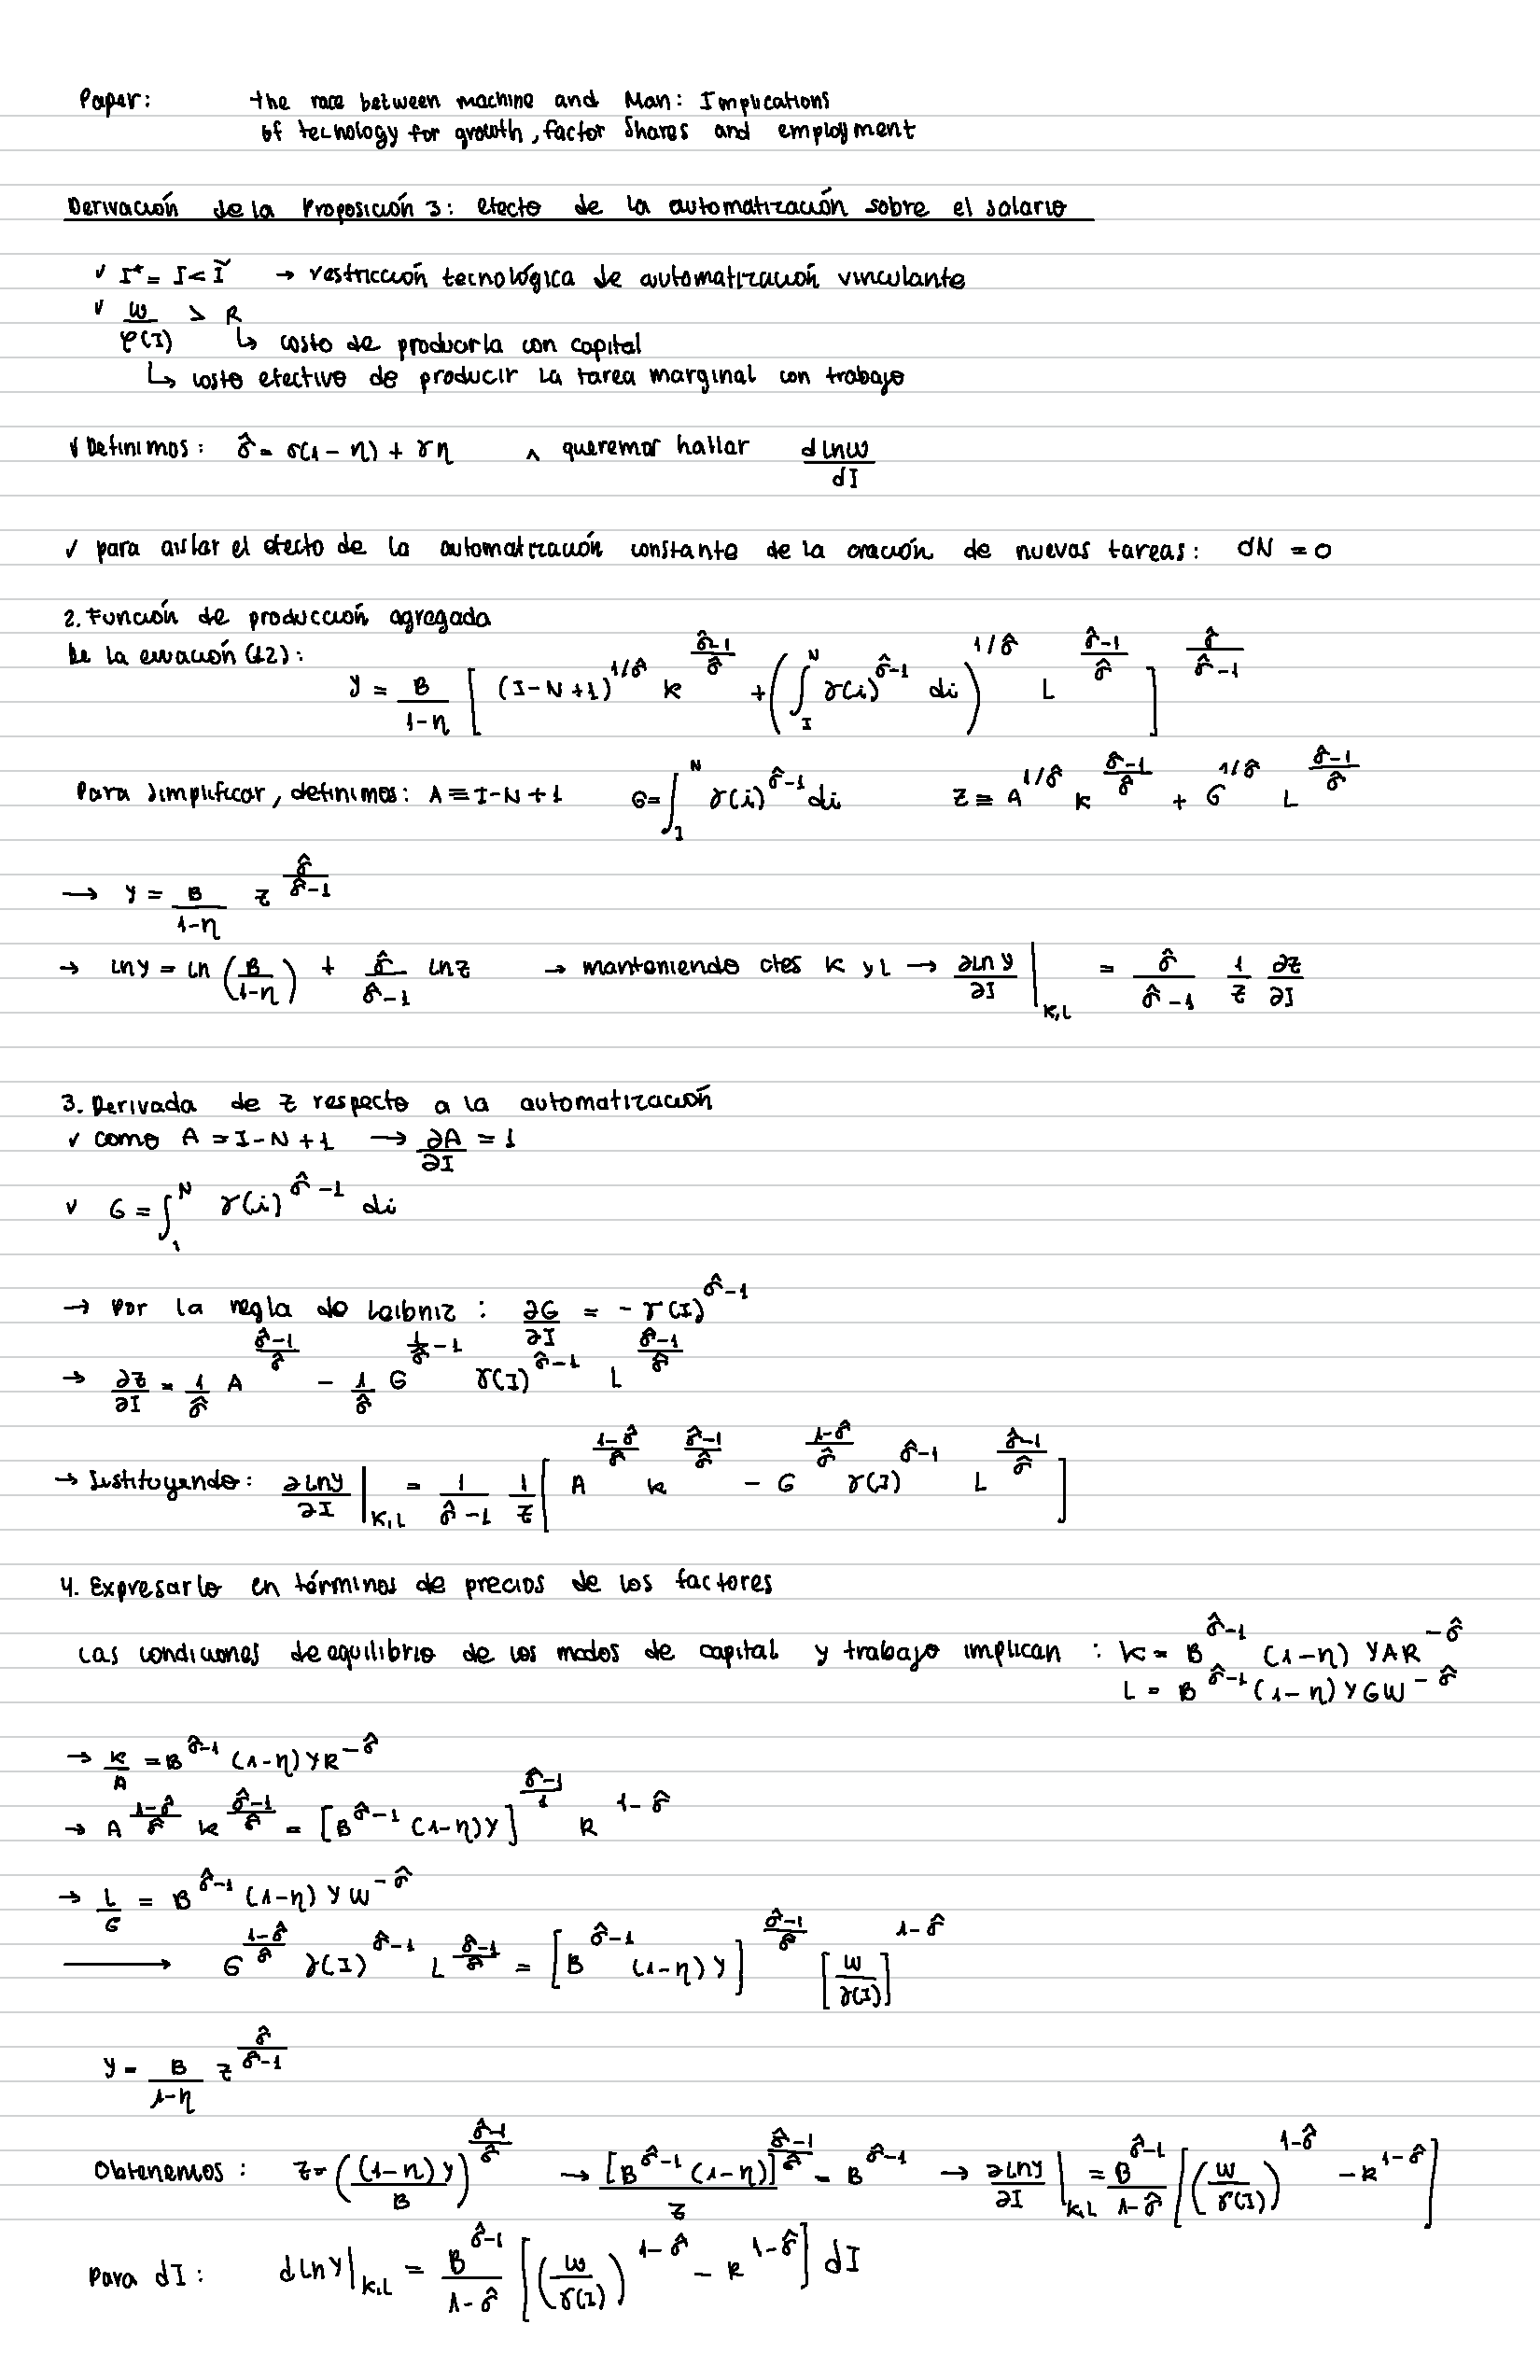
\includegraphics[page=1,width=\linewidth,height=0.62\textheight,keepaspectratio]{hand/Derivacion_manual_proposicion_3.pdf}

      {\scriptsize La hoja manual documenta el paso algebraico que luego se verifica en Lean.}
  \end{columns}
\end{frame}

\begin{frame}{Extensión: automatización en un intervalo intermedio}
  \centering
  \begin{tabular}{p{0.26\textwidth}p{0.26\textwidth}p{0.26\textwidth}}
    \cellcolor{teal!13}\centering Trabajo &
    \cellcolor{navy!12}\centering Capital &
    \cellcolor{teal!13}\centering Trabajo\tabularnewline
    $[N-1,I_L)$ & $[I_L,I_H]$ & $(I_H,N]$\tabularnewline
  \end{tabular}
  \vspace{0.65cm}
  \begin{itemize}
    \item La asignación deja de resumirse con un solo umbral.
    \item Automatizar una tarea en $I_L$ o en $I_H$ puede generar el mismo ahorro directo, pero un efecto agregado distinto.
    \item Cambian simultáneamente la masa de tareas por factor, la productividad y la sensibilidad de los precios relativos.
  \end{itemize}
  \vspace{0.35cm}
  \begin{block}{Predicción}
    La condición salarial conserva la lógica productividad versus desplazamiento, pero ambos términos pasan a depender de la ubicación de la tarea automatizada.
  \end{block}
  \source{Extensión propuesta en \texttt{extensions.md}.}
\end{frame}

\begin{frame}[fragile]{Lean: del sistema económico a una proposición verificable}
  \begin{columns}[T,onlytextwidth]
    \column{0.47\textwidth}
      \small
      \key{Afirmación matemática}
      \[
        \begin{gathered}
          s_Lw+(1-s_L)r=P_I\,dI,\\
          w-r=-D_I\,dI
        \end{gathered}
      \]
      implica
      \[
        w=[P_I-(1-s_L)D_I]dI.
      \]
      Si $dI>0$, entonces
      \[
        w>0\iff P_I>(1-s_L)D_I.
      \]
    \column{0.51\textwidth}
      \scriptsize
\begin{verbatim}
def propositionThreeWageEffectSpec : Prop :=
  forall sL PI DI dI w r : Real,
    0 < sL -> sL < 1 ->
    0 < PI -> 0 < DI -> 0 < dI ->
    sL*w + (1-sL)*r = PI*dI ->
    w-r = -DI*dI ->
    w = (PI-(1-sL)*DI)*dI /\
      (0 < w <-> (1-sL)*DI < PI)

theorem propositionThreeWageEffectProof :
    propositionThreeWageEffectSpec := by
  intro sL PI DI dI w r ...
  exact propositionThreeWageEffect ...
\end{verbatim}
  \end{columns}
  \source{\texttt{lean/PaperInterface.lean} y \texttt{lean/ProofInterface.lean}.}
\end{frame}

\begin{frame}{Qué verifica Lean y cuál es el límite}
  \begin{columns}[T,onlytextwidth]
    \column{0.48\textwidth}
      \begin{block}{Verificado}
        \begin{itemize}
          \item La solución exacta del sistema de dos ecuaciones.
          \item La equivalencia entre el signo salarial y la comparación de efectos.
          \item La prueba cierra sin \texttt{sorry}, axiomas temporales ni decisión nativa.
        \end{itemize}
      \end{block}
    \column{0.48\textwidth}
      \begin{block}{Fuera del alcance}
        \begin{itemize}
          \item Derivación de las ecuaciones desde la función de producción.
          \item Cálculo diferencial y umbral de capital.
          \item Resto de la Proposición 3 y resultados dinámicos.
        \end{itemize}
      \end{block}
  \end{columns}
  \vspace{0.35cm}
  \centering
  \textbf{Compilación:} \texttt{lake build +AR18RaceManMachine} aprobada.

  \textbf{Chequeo requerido:} \texttt{paper\_contribution.py check AR18RaceManMachine --fast} aprobado.
\end{frame}

\begin{frame}{Conclusiones}
  \begin{enumerate}
    \item La automatización reasigna tareas al capital. Por eso modifica productividad y distribución al mismo tiempo.
    \item En el caso restringido, la participación laboral cae, pero el salario depende del balance entre productividad y desplazamiento.
    \item La creación de nuevas tareas actúa en dirección opuesta y aumenta la demanda de trabajo.
    \item Lean confirma el núcleo algebraico de la condición salarial y deja explícito lo que todavía no se formalizó.
  \end{enumerate}
  \vspace{0.6cm}
  \centering
  {\Large\color{navy}\textbf{Preguntas}}
  \vspace{0.45cm}

  {\small Código, PDF y derivación: \href{https://github.com/isisroquet-mi/ai-06-restrepo}{github.com/isisroquet-mi/ai-06-restrepo}}
\end{frame}

\end{document}
